\section{Implementation}
Multiple popular derivative-free algorithms suited for specific scenarios exist \cite{rios2013derivative, paraskevoudis2020real, nevergrad}. The requirements for this scenario were determined as follows: 

\begin{enumerate}
    \item \textbf{The optimization problem is discrete.} A 3D printer's accuracy is limited and thus discrete. For example, the print temperature might be set to 221.20348129344\textdegree C but 3D printers are not capable of printing such fine-grained settings. Even though a print temperature of 221.20348129344\textdegree C might be set, a printer would print with 221\textdegree C.
    \item \textbf{The optimization problem has constraints.} Print settings have known constraints in which the optimum lays. Testing a print temperature below 150\textdegree C is unnecessary. The plastic will not reach the melting point and thus can not be printed. Similarly, a print temperature above 250\textdegree C will lead to worse quality.
    \item \textbf{A surrogate model-based optimizer is required.} How "good" or "bad" certain print settings are can only be observed through the users ranking of previous prints and can not be measured directly. A surrogate-based optimizer approximates the objective of better print settings, not to confuse with the objective function which is the user's ranking, through previously observed evaluations (test prints)\cite{karlsson2020continuous, molnar2019}. The key difference to non-surrogate optimizers is the fact that the choices of observations are optimized, not the evaluation itself. In the context of this paper: The choice of which print settings to test next is optimized, not the objective of better print settings itself. But by optimizing the choices, "good" print settings can be approximated \cite{molnar2019}. One can think of surrogate-based optimizers as optimizers that make informed guesses (choices) where the optimum (good print settings) might lie.  
    \item \textbf{The optimizer needs to yield results with as few evaluations as possible.} This optimization problem's bottleneck is printing time and required manual labor. Each evaluation takes at least 10 minutes, dependent on the test object. It follows that as little as 6 evaluations easily take one hour to proceed while additionally requiring manual labor to set up each evaluation print. 
\end{enumerate}

Requirements 3 and 4 go hand in hand. Surrogate models, also known as approximation models, are mainly used to reduce the number of evaluations of an objective function \cite{molnar2019}. Therefore, the choice for the optimization algorithm boils down to a surrogate-based optimizer that can optimize constrained discrete parameters. One of the investigated optimization algorithms was Bayesian optimization. Bayesian optimization utilizes a Gaussian process that provides a probability distribution as a surrogate model for the objective (of better print settings) in combination with an acquisition function \cite{frazier2018tutorial}. The purpose of the acquisition function is to determine which values to sample next i.e. which print settings to test next based on the probability distribution. The acquisition functions exploration and exploitation trade-off can be influenced through the hyperparameters xi $\xi$ and kappa $\kappa$ \cite{agnihotri2020exploring, bayesianPythonPackage}. $\xi$, $\kappa$ and the choice of the acquisition function itself modify the probability distribution which in turn adjusts the exploration and exploitation behaviour of the optimizer \cite{agnihotri2020exploring}. After each evaluation (test print), the probability distribution is updated to account for the new evaluation \cite{frazier2018tutorial, agnihotri2020exploring}. The process is repeated for a specified amount of epochs. Figure \ref{figure/bayesian_optimization_illustration} illustrates the process of Bayesian optimization. While Bayesian optimization is of continuous nature, since the underlying probability distribution is continuous, recent research has found Bayesian optimization to perform well on discrete problems as well, even outperforming state-of-the-art discrete optimization algorithms \cite{karlsson2020continuous}. Initial tests have shown that Bayesian optimization approximates optimal print settings in a simulated environment relatively fast and consistently. Furthermore, in comparison to other algorithms, an excellent Python package from Fernando Nogueira that implements the algorithm with an extendable API exists \cite{bayesianPythonPackage}. Because of the promising initial tests compared to other optimization algorithms \footnote{The compared-to algorithms were mostly from the Nevergrad package. Nevergrad is a Python package developed by Facebook Research that labels itself as a gradient-free optimization platform \cite{nevergrad}. The appeal of the package is bundling multiple optimization algorithms in one package, all wrapped with a single API. The single API makes testing of different algorithms with little duplicated, or adjusted, code possible.}, the recent research indicating that Bayesian optimization outperforms dedicated discrete optimizers and the available Python package, bayesian optimization has been chosen as the optimization algorithm for this project. 


\begin{figure*}[!htb]
    \centering
    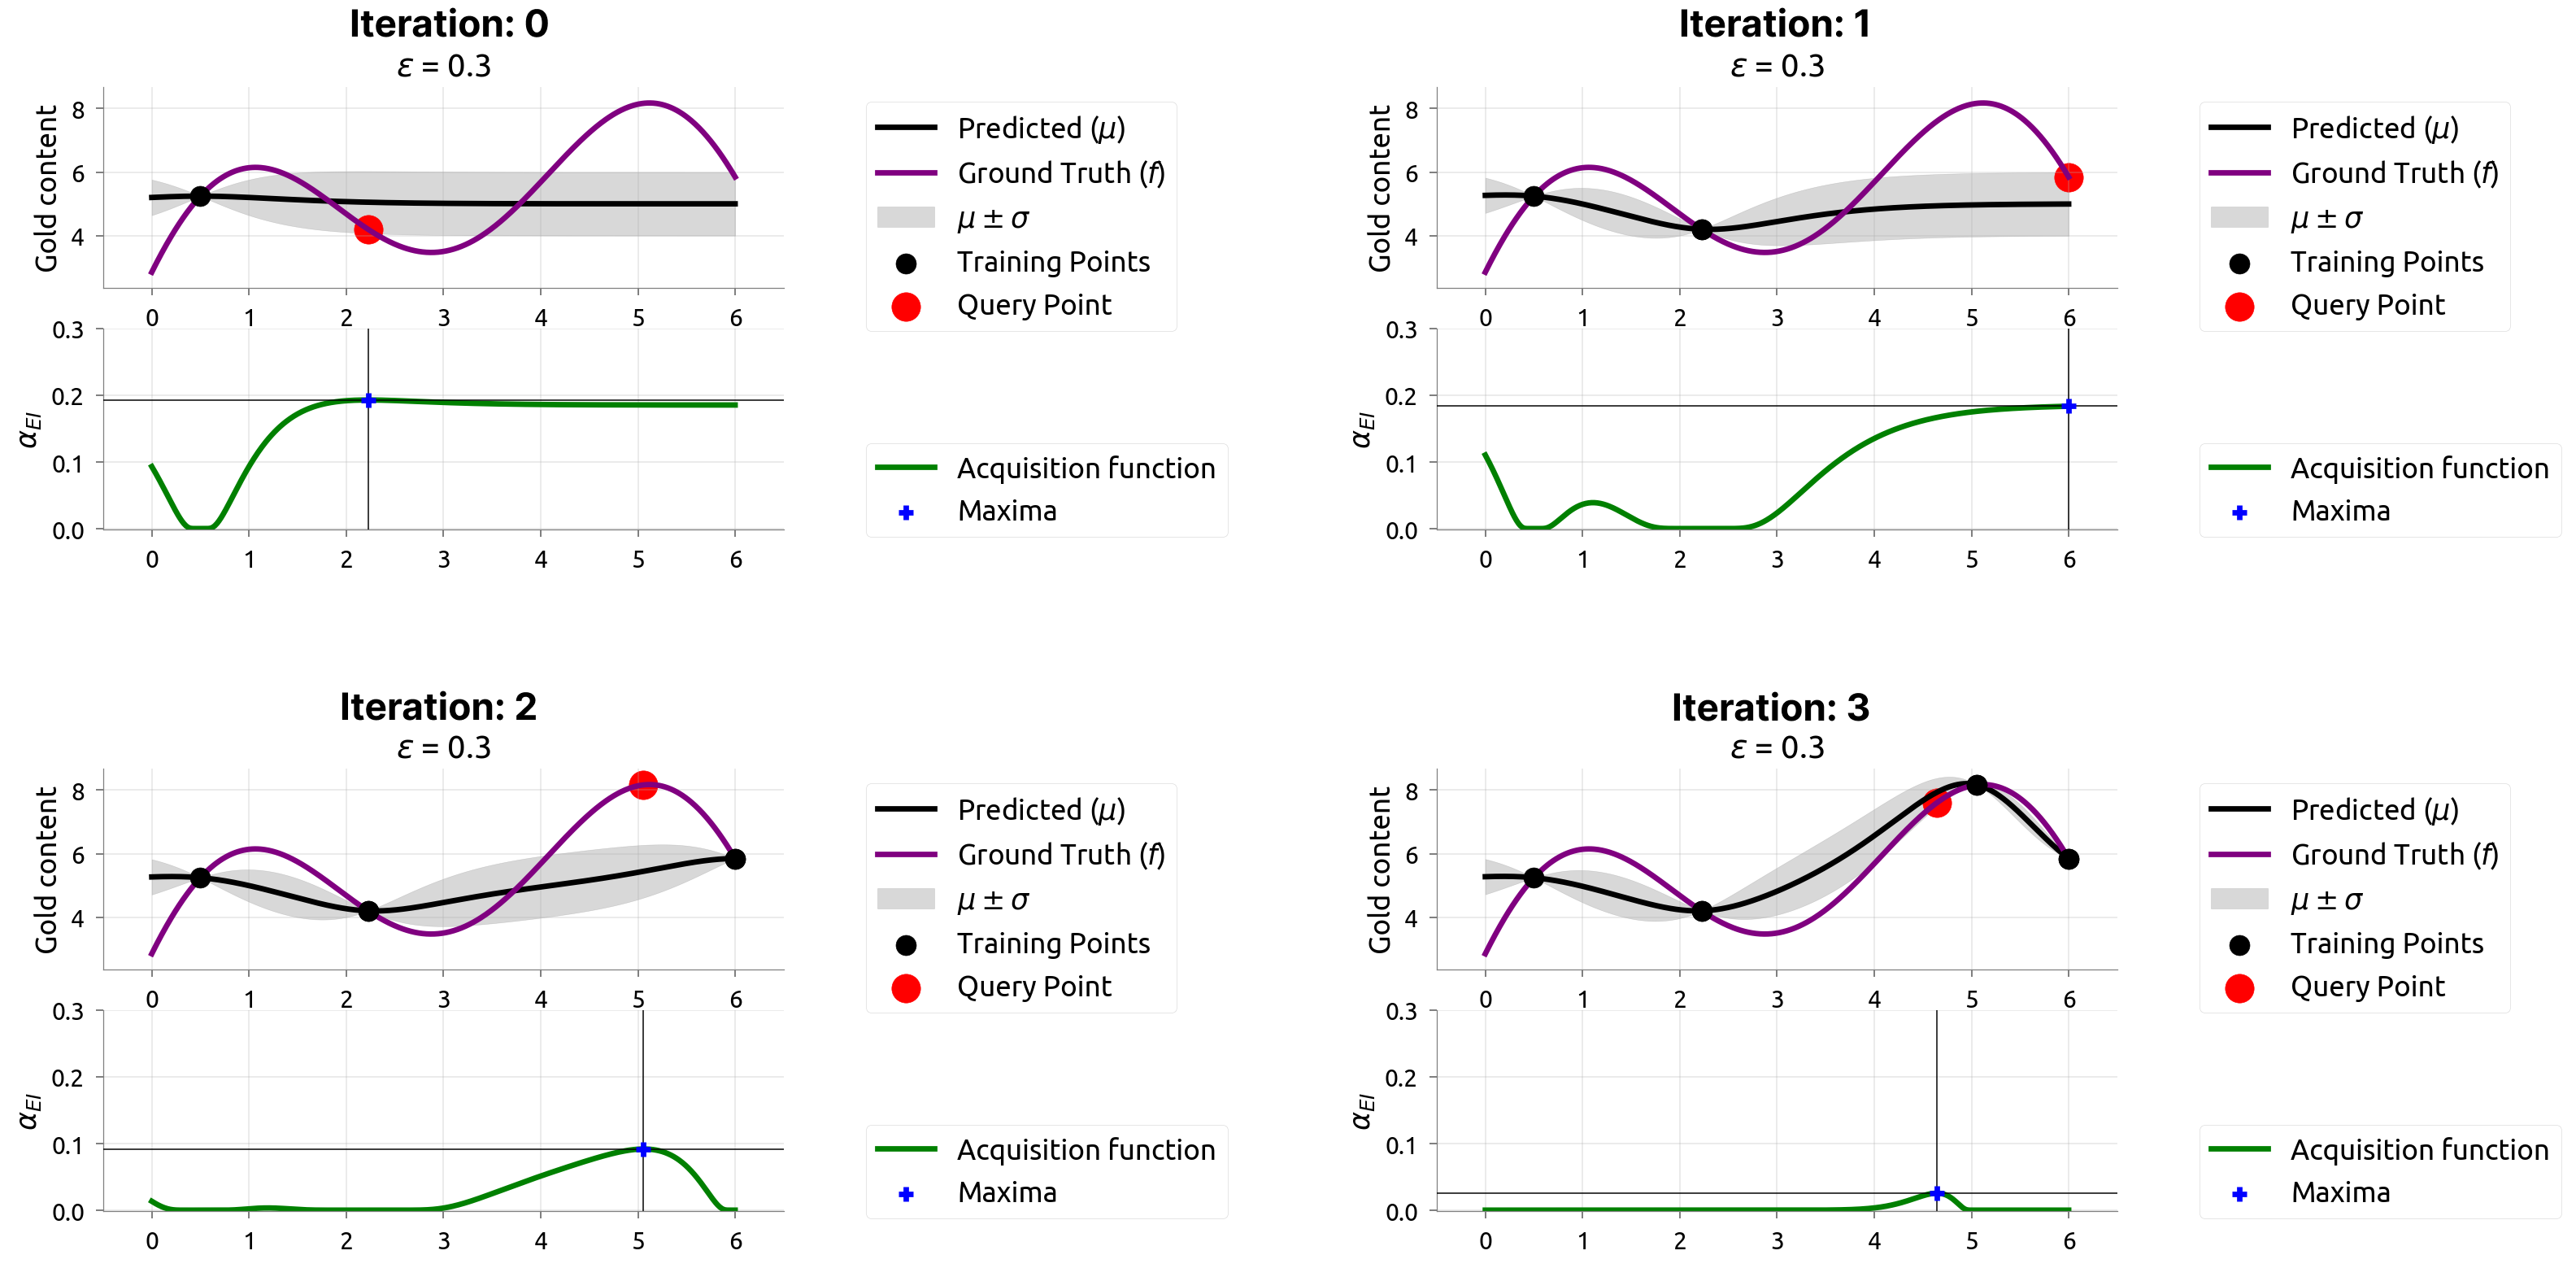
\includegraphics[width=\textwidth]{assets/bayesian_optimization_illustration.png}
    \caption{An exemplary Bayesian optimization process. Iteration 0 is the start of the process where one point has been evaluated at $x\approx0.5$. The acquisition function's maximum is at $x\approx2.2$. Therefore, in the next iteration (iteration 1), the evaluated point is $x\approx2.2$. After the evaluation of $x\approx2.2$ the probability distribution is updated and the next point, as determined by the acquisition function, is evaluated. The plots show how Bayesian optimization improves the approximation of the objective with each iteration. The objective is shown as \textit{Ground Truth} in the plots, while the approximation is shown as \textit{Predicted}. The plots were taken from Agnihotri & Batra, "Exploring Bayesian Optimization", Distill, 2020 \cite{agnihotri2020exploring}.}
    \label{figure/bayesian_optimization_illustration}
\end{figure*}

\subsection{Adjusting Bayesian Optimization for Discrete Values}
Although Bayesian optimization can work with discrete values, the implementation from Fernando Nogueira does not support discrete values \cite{bayesianPythonPackage}. Fernando Nogueira himself proposed a simple float to integer cast in the GitHub repository \cite{bayesianPythonPackage} which is in line with other research \cite{garrido2020dealing}. The question arises where to cast or round to an integer within the implementation. Garrido-Merchán et al. suggest three approaches \cite{garrido2020dealing}: 
\begin{enumerate}
    \item Within the step e.g. which point to sample next.
    \item Within the objective function.
    \item Inside the Gaussian process.
\end{enumerate}

Modifying the Gaussian process performed best in the experiments conducted by Garrido-Merchán et al. \cite{garrido2020dealing}. However, that observation was influenced by the fact that hyper-parameter tuning was deemed too expensive. Without appropriate hyper-parameters, the first approach, which is easier to implement, might result in the convergence process "getting stuck" in a local optimum \cite{garrido2020dealing}. But, hyper-parameter tuning is easily conducted in this project using a simulated environment that avoids real prints. Without real test prints, the optimization problem becomes "cheap" (time-wise, computationally it is cheap regardless of a simulated environment or not), allowing for exhaustive automated hyper-parameter tuning, diminishing the downside of approach 1 while keeping the benefit of easier integration. The second approach of casting or rounding continuous values to a discrete value within the objective function is easiest to implement but tests have shown that the approach did not work in combination with the following improvement developed during testing: 

To further reduce the number of evaluations, and by that improve upon requirement 4, the probes are binned to defined step sizes. Binning refers to grouping a set of numbers "together". For example, no notable difference between one-degree print temperature e.g. 205\textdegree C and 206\textdegree C is visible. \begin{wrapfigure}{r}{0.44\textwidth}
    \centering
    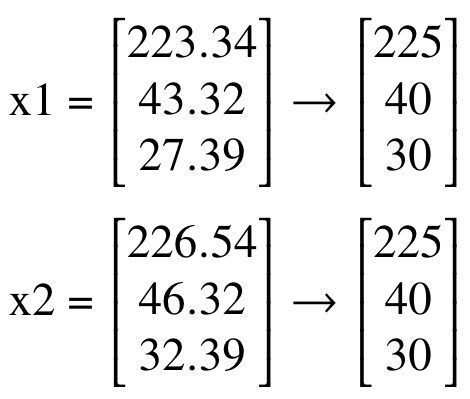
\includegraphics[width=0.9\linewidth]{assets/casting_binning_matrices.png}
    \caption{Two exemplary probed points $x1$ and $x2$ and their output after binning, also illustrating the potential problem of probed points being binned to the "same" point.}
    \label{figure/casting_binning_matrices}
\end{wrapfigure} Therefore, suggesting unnoticeable differences and by that "wasting" evaluations is reduced by defining step sizes for print settings. Each sample that the acquisition function then chooses is "binned" to the closed step size. Print temperatures might be binned as following: The step size is set to 5\textdegree C. The optimizer then probes temperatures in the given constraints e.g. 180\textdegree C to 220\textdegree C which could yield 186.21\textdegree C. The binning process then rounds 186.21\textdegree to the closet value of the defined step size of 5 which results in 185\textdegree C. In the given example, binning reduces the number of probable temperature settings by a factor of 5 from 40 to 8. The drastic reduction of probable settings came with a downside: testing revealed that although the optimizer yielded results much faster, the optimizer oftentimes "got stuck" probing different points which are binned to the same point. Figure \ref{figure/casting_binning_matrices} shows an illustration of the problem binning can entail. To solve the problem, temporarily adjusting the optimizer's hyper-parameters $\xi$ and $\kappa$ to increase exploration, if the current probe is identical to an already probed point, has been tested. Unfortunately, the method has been found to have a neglectable effect. Since the alternative of stopping the optimization process upon sampling an identical probe has led to unoptimized print settings, an alternative to dynamically adjusting the exploration of the optimizer had to be found. The solution was simple: If a newly sampled probe is identical to an already probed sample, sample a new random probe until the obtained random sample is not identical to an already probed sample.

Coming back to why the second approach did not work: Due to binning, casting/rounding within the objective function lead the optimization process to "get stuck", regardless of the random sampling solution. Reason being that the binned probed points are internally saved as unbinned continuous probes. With each step, the acquisition function takes the unbinned probes into account to sample a new probe. But the differences between the unbinned and evaluated probes vastly differ, unbeknown to the optimizer. Ultimately, modifying the sampling method (approach 1) has been chosen because it was easier to implement compared to modifying the Gaussian process and worked with binning.


\subsection{Simulation and Hyperparameter Tuning}

% 1. Using ranking -> points chosen by objective function v3 
% 2. each run = 100 times with different TRUTH VALUE for each run 
% 3. each run has epochs = 10 + 2 (mehr ist nicht zumutbar)
% 4. median from each run for best solution is taken saved in combination with the loss
% 5. NAIVE approach -> test all hyper-parameter combinations as cheap to compute
% 6. hyper-parameters with lowest median wins

The convergence of Bayesian optimization depends on the chosen acquisition function and the functions hyper-parameters \cite{agnihotri2020exploring}. Since this optimizations problems bottle-neck is the time it takes to print test objects and not computational resources, a simulated environment has been developed which allows for cheap(er) hyper-parameter tuning. 

\subsubsection{Print Settings of Focus (The Parameters)}
Theoretically, the chosen and modified bayesian optimization algorithm should be able to optimize any print setting, as long as visible differences for the to-be-optimized print setting are visible to the user during the evaluation/ranking step. However, the simulation, and later the evaluation of the implementation is conducted focusing on print settings that have been identified as over-proportionally influential and simultaneously relatively fast testable with a specific object \cite{paraskevoudis2020real, teachingTechCalibration}. The parameters, including their constraints and step size, given as (lower bound, higher bound, step size), are: 
\begin{enumerate}
    \item \textbf{Print Temperature \textit{in \textdegree C} (180, 220, 5):} Determines the extrusion temperature i.e. at which temperature the plastic should be extruded. If the temperature is too low, layers do not stick together. If the temperature is too high, the viscosity of the extruded plastic is too low leading to diminishing print quality.
    \item \textbf{Retraction Distance \textit{in mm} (2, 8, 1):} An illustration and detailed explanation is given in figure \ref{figure/stringing}.
    \item \textbf{Flow Rate \textit{in \%} (90, 110, 2):} Determines how much plastic should be extruded. Extruding not enough plastic leads to under-extrusion that is visible by gaps in the object. Extruding too much plastic results in over-extrusion visible by surface defects such as blobs. Figure \ref{figure/extrusion_example} shown an illustration of under- and over-extrusion.
\end{enumerate}

\textit{The constraints, step sizes and description have been defined or chosen through multiple years of experience and various online resources such as \cite{printTemperatureSetting, flowRateSetting}.} 

\begin{figure}[h]
    \centering
    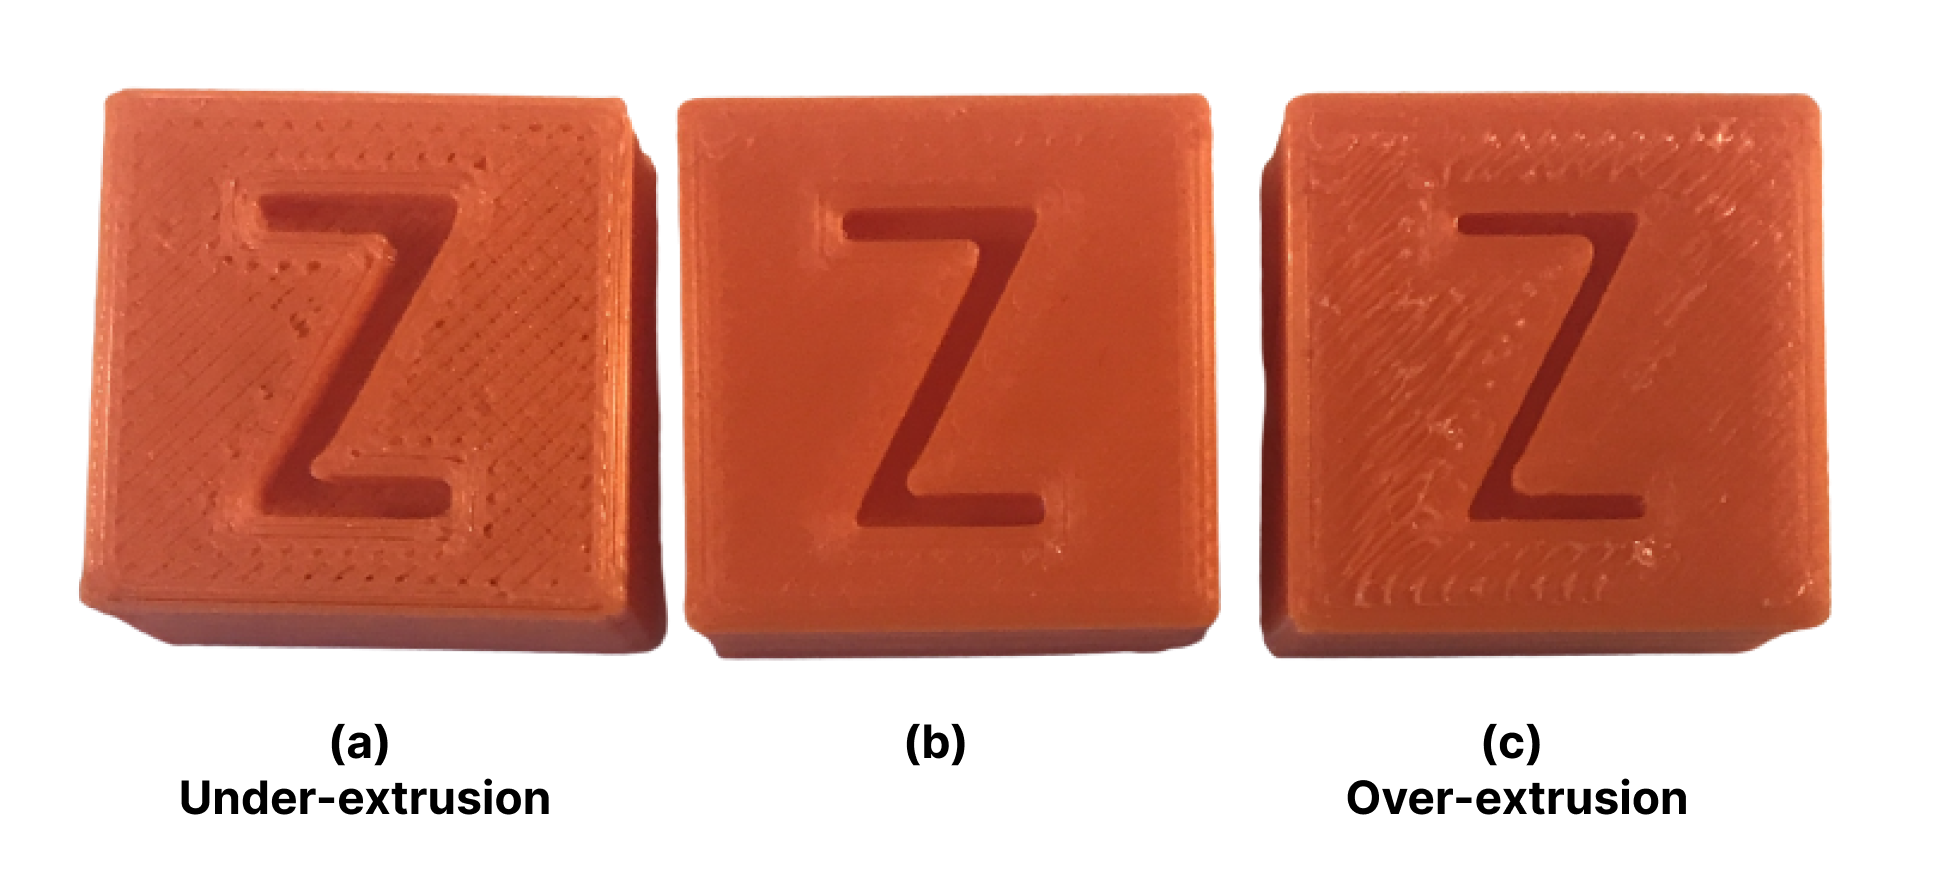
\includegraphics[width=0.7\linewidth]{assets/extrusion_example.png}
    \caption{Illustration of the effect flow rate can have on the print quality. In particular, a too low flow rate leads to under-extrusion as shown in (a), while a high flow rate can lead to over-extrusion as shown in (c). A relatively good flow rate and corresponding print quality are shown in (b).}
    \label{figure/extrusion_example}
\end{figure}

\subsubsection{Loss Function}

To simulate an optimization process, the objective function i.e. the ranking of print settings needs to be simulated. And to simulate the ranking of print settings, a loss function determining how "good" or "bad" given print settings (parameters) are, had to be developed. The developed loss function sums the absolute distance of each given parameter to a truth value divided by the parameters step size. The division by the parameters step sizes adjusts potential weight imbalances between parameters with different step sizes. Lastly, the sum is multiplied by -1 since the optimizer is maximizing. The result is a loss function that sums each of the parameter's deviation from the truth value under consideration of the step size by -1. A concrete example loss calculation is shown in figure \ref{figure:loss_function_example} and pseudocode of the implementation in figure \ref{figure/loss_function_pseudocode}. 
\begin{figure}[h]
    \centering
    \begin{minted}{javascript}
    function loss(parameters, step_sizes, truth_value):
        results = empty list
        for index in length(parameters):
            calculation = absolute((truth_value[i] - parameters[i]) / step_sizes[i])
            results.add(calculation)
        return -1 * sum(results)
    \end{minted}
    \caption{Pseudocode illustrating the implementation of the loss function.}
    \label{figure/loss_function_pseudocode}
\end{figure}

\begin{figure}
    \centering
    \[parameters =  \begin{bmatrix}
    210 \\
    5 \\
    30 
    \end{bmatrix}, 
    truth values = \begin{bmatrix}
    215 \\
    3 \\
    50 
    \end{bmatrix},
    step sizes = \begin{bmatrix}
    5 \\
    1 \\
    10 
    \end{bmatrix}
    \]
    \begin{align} 
    &=  abs(\begin{bmatrix}
    210 \\
    5 \\
    30 
    \end{bmatrix} -
    \begin{bmatrix}
    215 \\
    3 \\
    50 
    \end{bmatrix}) \div
    \begin{bmatrix}
    5 \\
    1 \\
    10 
    \end{bmatrix} \\
    &= \begin{bmatrix}
    5 \\
    2 \\
    20 
    \end{bmatrix} \div \begin{bmatrix}
    5 \\
    1 \\
    10 
    \end{bmatrix} \\
    &= sum(\begin{bmatrix}
    1 \\
    2 \\
    2 
    \end{bmatrix}) \\
    &= -1 * 5 \\
    &= -5
    \end{align}
    
    \caption{Pseudo algebra showcasing the calculation of the loss function. $Parameters$ corresponds to the probed point. The calculation showcases weight adjustments of parameters with different step sizes. The first parameter $210$ is $5$ apart from the truth value $215$ but the step size for this parameter is $5$, thus the probed parameter is only $1$ "step size" apart from the truth value. All parameters in sum are $5$ step sizes apart from the truth values. Therefore, the loss is $5 *-1 = -5$ (because of maximization; the perfect loss is 0).}
    \label{figure:loss_function_example}
\end{figure}    


\subsubsection{User Ranking (The Objective Function)}
The ranking process is straightforward: The better the print, the higher its rank. After each print, the user is asked to determine the rank of the new print. The process might look as following: The user has printed 3 test objects, each with different print settings, which are stacked on top of each other. The bottom print has the rank 0, the middle print rank 1, and the upper print rank 2. A new test print might be ranked as 2. In that case, the new print is inserted below the upper print in the stack. After each ranking, the optimizer is re-initialized to take the new and adjusted ranks into account.

The simulation of the user ranking is also straightforward: Instead of asking a user to rank the print, the loss of a print, as returned by the loss function, determines its rank. 

\newpage
\subsubsection{Simulated Optimization Process}

The hyperparameters to optimize are the choice of the acquisition function, kappa $\kappa$ and xi $\xi$. For all of the following simulations, the number of epochs has been set to 18 plus 2 for the initial probes.  Expecting a user to print more than 20 test prints seems unreasonable. Furthermore, in each run, a random truth value is generated to simulate different printers which are assumed to have different optimal print settings. It is important to note that the random truth value does account for the constraints but does not account for the step sizes. Thus, the truth value might be "unreachable" for the optimizer given certain step sizes. For example, the truth value for the print temperature might randomly be chosen as 203. If the step size of the print temperature is defined to be 5, then the optimizer can only probe 200 or 205 but not 203. For the simulation, this effect was determined to be not harmful and likely resembles real application. One run is defined as one optimization process which in itself has 18 plus 2 epochs. Thus, 10 runs lead to the generation of 10 different truth values which the optimizer is set to optimize in 18 plus 2 epochs. 

One of the solutions tested in response to the earlier mentioned binning problem was to statically set the first two probes as lower- and higher bound of the determined constraints. An example: The constraints are set as lower bound: (190,5,20) and higher bound (220,10,60). The first two probed points are then [190,5,20] and [220,10,60]. Although the binning problem was solved using random sampling, the effects of static or random initial probes have been tested. The results revealed that both the median and mean loss are lower, thus better, using random initial probes. To reduce the time complexity of further simulations, random initial probes are used and further evaluation of static initial probes has been omitted. 

Afterwards, a simulation has been conducted to determine which acquisition function could be excluded from further simulations and to narrow the range of tested $\xi$ and $\kappa$ parameters. Reason being that although this optimization problem is computationally cheap(er), performing naive hyperparameter tuning by simulating all possible combinations results in bad time complexity and therefore long running time. The range of $\kappa$ has been set to 0 to 10 with a step size of 1. The range of $\xi$ been set to 0 to 1 with a step size of 0.1. Both the $\kappa$ and $\xi$ range has been set in accordance with explanations provided by Nogueira \cite{bayesianPythonPackage}. Each unique combination of the hyperparameters has been simulated 10 times. The result is shown in figure \ref{figure/experiment2}. Across all acquisition functions, the mean loss was higher than -2. Remember that 0 is the absolute best the optimizer can achieve whereas -2 means the optimizer is two-step sizes away from the optimal solution. Regardless, the Expected Improvement (ei) acquisition function slightly outperformed the other acquisition functions and has therefore solely been selected for simulation runs. Furthermore, the optimal $\kappa$ value seems to lay in between 1 and 4 while the optimal $\xi$ value seems to lay above 0.5 potentially exceeding the set bound of 1. 

\begin{figure}%
\centering
\subfigure[Grouped by acquisition function]{%
\begin{tabular}{lr}
\toprule
{} &  mean loss \\
acquisition function &            \\
\midrule
ei                   &      -1.22 \\
poi                  &      -1.83 \\
ucb                  &      -1.57 \\
\bottomrule
\end{tabular}}
\qquad
\subfigure[Ei acquisition function mean loss grouped by kappa]{%
\begin{tabular}{lr}
\toprule
{} &  mean loss \\
kappa &            \\
\midrule
0     &      -1.33 \\
1     &      -1.33 \\
2     &      -1.16 \\
3     &      -1.28 \\
4     &      -1.14 \\
5     &      -1.07 \\
6     &      -1.21 \\
7     &      -1.23 \\
8     &      -1.22 \\
9     &      -1.20 \\
\bottomrule
\end{tabular}
}
\qquad
\subfigure[Ei acquisition function mean loss grouped by xi]{%
\begin{tabular}{lr}
\toprule
{} &  mean\_loss \\
xi  &            \\
\midrule
0.0 &      -1.41 \\
0.1 &      -1.45 \\
0.2 &      -1.21 \\
0.3 &      -1.27 \\
0.4 &      -1.05 \\
0.5 &      -1.12 \\
0.6 &      -1.22 \\
0.7 &      -1.21 \\
0.8 &      -1.07 \\
0.9 &      -1.15 \\
\bottomrule
\end{tabular}}
\caption{Results of the second simulation: Table (a) shows the mean loss of the acquisition functions over 300 runs with different xi and kappa values whereas each unique combination has been repeated 10 times, totaling the number of runs to 3000. Table (b) and (c) show the mean loss of the different kappa $\kappa$ and xi $\xi$ values for the Expected Improvement "ei" acquisition function. }
\label{figure/experiment2}
\end{figure}

One last simulation has been conducted to determine the optimal $\kappa$ and $\xi$ value for the Expected Improvement acquisition function. The range of $\kappa$ has been further narrowed from 0 to 10 \textit{to} 1 to 6 while the range of $\xi$ has been been shifted from 0 to 1 \textit{to} 0.5 to 1.5. The reduced computing time caused by lowering the number of acquisition functions and narrowing the $\kappa$ value was used to increase the number of runs per rotation from 10 to 100. The increased number of runs should reduce the influence of the randomized initial points and random samples caused by the binning process. All runs had a mean loss higher than -2. In contrast to the previous simulations, the median of the number of epochs until the best solution has been found was evaluated besides the mean loss of the best solution. Reason being, the earlier the optimizer finds the best solution, the fewer prints have to be conducted. Figure \ref{figure/simulation3} shows a subset of the results. Based on the result, the optimal hyperparameters have been chosen as the Expected Improvement acquisition function with $\kappa$ = 1 and $\xi$ = 0.7.

\begin{figure}
    \centering
    \begin{tabular}{rrrr}
    \toprule
     kappa &  xi &  median epochs until best solution &  mean loss \\
    \midrule
         1 & 0.7 &                  13.0 &     -0.973 \\
         3 & 1.1 &                  13.0 &     -1.009 \\
         2 & 1.2 &                  15.0 &     -1.027 \\
         1 & 0.8 &                  13.0 &     -1.055 \\
         2 & 0.6 &                  14.0 &     -1.058 \\
    \bottomrule
    \end{tabular}
    \caption{Top 5 results of the third simulation sorted in ascending order by the mean loss.}
    \label{figure/simulation3}
\end{figure}